\documentclass[11pt,border=10pt]{standalone}
\usepackage{tikz}
\usepackage{hyperref}
\hypersetup{hidelinks}
\usetikzlibrary{shadows,arrows}
\usepackage[final]{fixme}
\fxsetup{layout=footnote, marginclue}
\usepackage{pdfbase}[2017/03/16]
\usepackage{xparse,ocgbase}
\usepackage{xcolor,calc}
\usepackage{tikzpagenodes,linegoal}
\usetikzlibrary{calc}
\usepackage{pdfcomment}
\usepackage{soulpos}
\usepackage{amsmath}



% Define the layers to draw the diagram
\pgfdeclarelayer{background}
\pgfdeclarelayer{foreground}
\pgfsetlayers{background,main,foreground}


% Define block styles  
\tikzstyle{materia}=[draw, fill=blue!5, text width=6.0em, text centered,minimum height=1.5em,drop shadow]
\tikzstyle{fuellung}=[draw, fill=green!15, text width=12.0em, text centered,minimum height=1.5em,drop shadow]
\tikzstyle{beruffuell}=[draw, fill=red!15, text width=30.0em, text centered,minimum height=2em,drop shadow]
\tikzstyle{dummi}=[draw, fill=red!50, text width=1.0em, text centered,minimum height=1em,drop shadow]
\tikzstyle{practica} = [materia, text width=15em, minimum width=17em,minimum height=3em, rounded corners, drop shadow]
\tikzstyle{beruf} = [beruffuell, text width=90em, minimum width=10em,minimum height=10em, rounded corners, drop shadow]
\tikzstyle{abschl} = [fuellung, text width=15em, minimum width=16em,minimum height=3em, rounded corners, drop shadow]
\tikzstyle{dumm} = [dummi, text width=1em, minimum width=1em,minimum height=1em, rounded corners, drop shadow]
\tikzstyle{texto} = [above, text width=10em, text centered]
\tikzstyle{linepart} = [draw, thick, color=black!50, -latex', dashed]
\tikzstyle{line} = [draw, thick, color=black, -latex']
%\tikzstyle{ur}=[draw, text centered, minimum height=0.01em]

% Define distances for bordering
\newcommand{\blockdist}{1.3}
\newcommand{\edgedist}{1.5}

\newcommand{\practica}[2]{node (p#1) [practica]	{{\textbf{#2}}}}
\newcommand{\abschl}[2]{node (p#1) [abschl]	{{\textbf{#2}}}}
\newcommand{\beruf}[2]{node (p#1) [beruffuell]	{{\textbf{#2}}}}
\newcommand{\dumm}[2]{node (p#1) [dumm]	{{\textbf{#2}}}}
\newcommand{\abstand}{3.5cm}
\newcommand{\abstandv}{5cm}
\newcommand{\abstandvv}{1cm}

\newcommand{\transreceptor}[3]{%
	\path [linepart] (#1.east) -- node [above]
	{\scriptsize Transreceptor #2} (#3);}

\begin{document}
	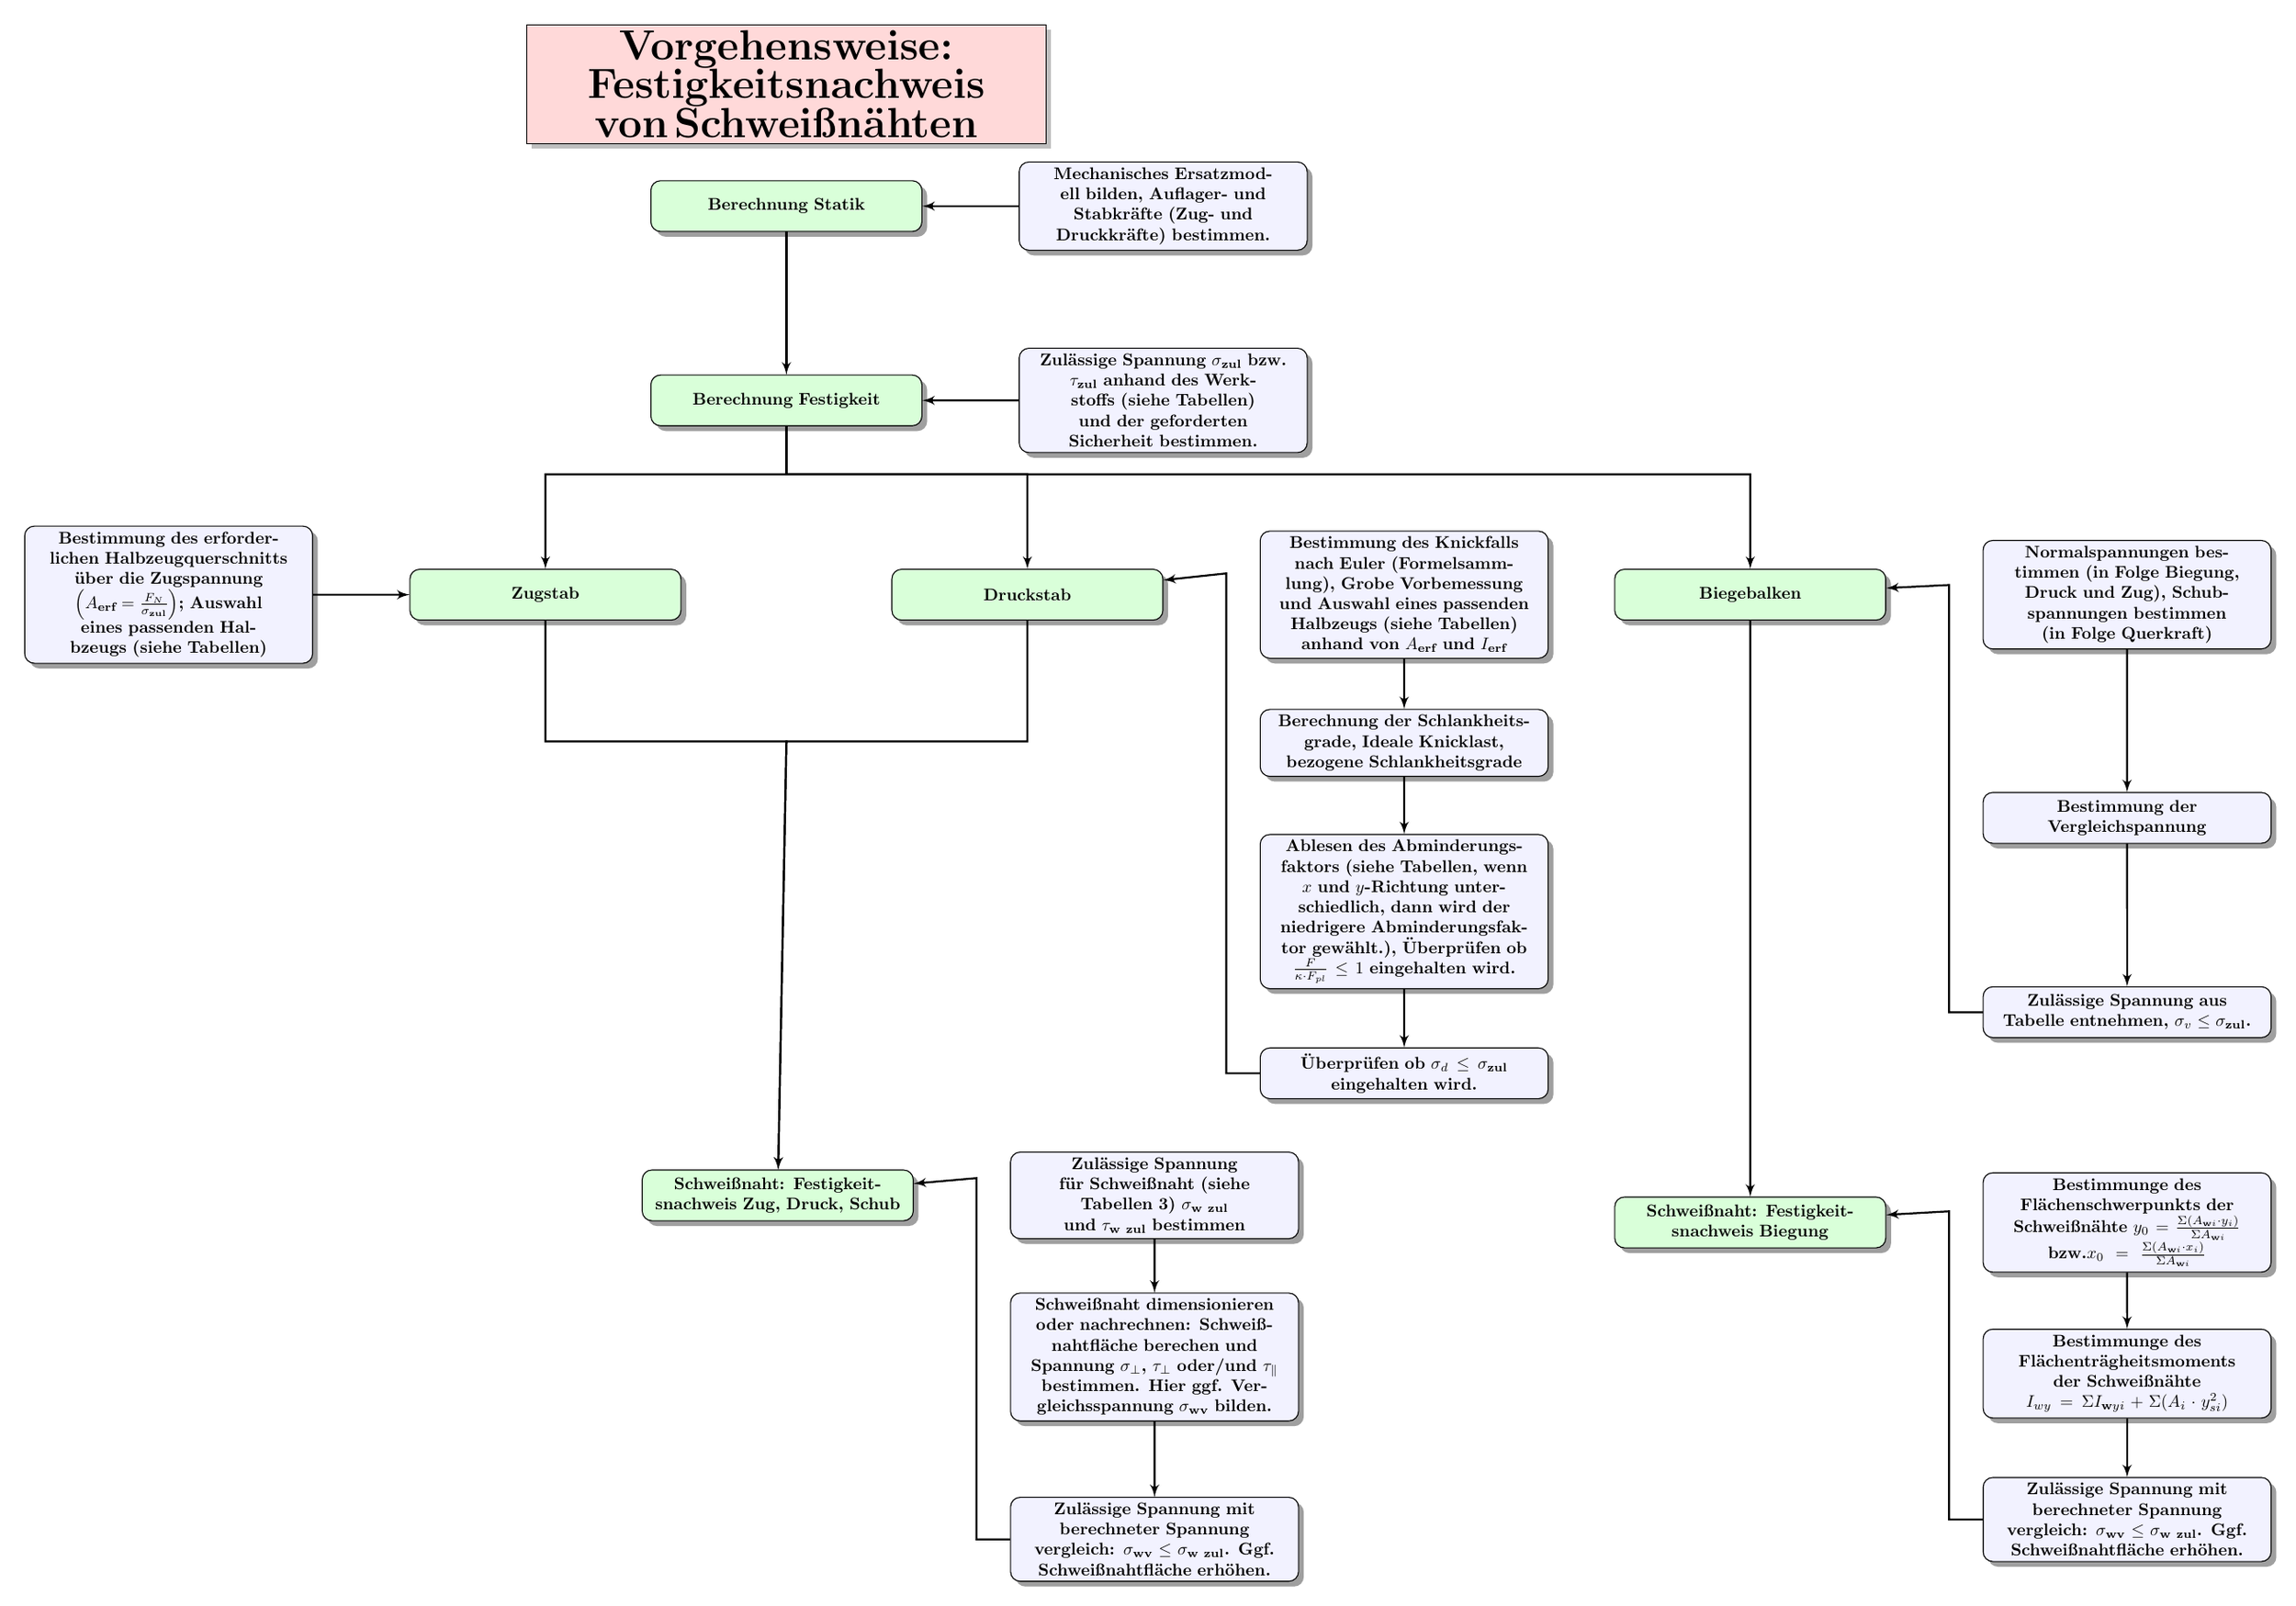
\begin{tikzpicture}[scale=0.7,transform shape]
	
	% Draw diagram elements
	
	\path \abschl {1}{Berechnung Statik};
	\path (p1.north)+(0,2) \beruf{80}{\Huge Vorgehensweise: Festigkeitsnachweis von Schweißnähten};
	\path (p1.east)+(\abstandv,0) \practica {2}{Mechanisches Ersatzmodell bilden, Auflager- und Stabkräfte (Zug- und Druckkräfte) bestimmen.};
	
	%Festigkeit
	\path (p1.south)+(0,-\abstand)\abschl {3}{Berechnung Festigkeit};
	\path (p3.east)+(\abstandv,0) \practica {4}{Zulässige Spannung $\sigma_{\text{zul}}$ bzw. $\tau_{\text{zul}}$ anhand des Werkstoffs (siehe Tabellen) und der geforderten Sicherheit bestimmen. };
	
	%Zugstäbe
	\path (p3.south)+(-\abstandv,-\abstand)\abschl {7}{Zugstab};
	\path (p7.west)+(-\abstandv,0) \practica {8}{Bestimmung des erforderlichen Halbzeugquerschnitts über die Zugspannung $\left(A_{\text{erf}}=\frac{F_N}{\sigma_{\text{zul}}}\right)$; Auswahl eines passenden Halbzeugs (siehe Tabellen)};
	
	%Druckstäbe
	\path (p3.south)+(\abstandv,-\abstand)\abschl {9}{Druckstab};
	\path (p9.east)+(\abstandv,0) \practica {10}{Bestimmung des Knickfalls nach Euler (Formelsammlung), Grobe Vorbemessung und Auswahl eines passenden Halbzeugs (siehe Tabellen) anhand von $A_{\text{erf}}$ und $I_{\text{erf}}$};
	\path (p10.south)+(0,-.5*\abstand) \practica {11}{Berechnung der Schlankheitsgrade, Ideale Knicklast, bezogene Schlankheitsgrade};
	\path (p11.south)+(0,-.8*\abstand) \practica {12}{Ablesen des Abminderungsfaktors (siehe Tabellen, wenn $x$ und $y$-Richtung unterschiedlich, dann wird der niedrigere Abminderungsfaktor gewählt.), Überprüfen ob $\frac{F}{\kappa\cdot F_{pl}}\leq 1$ eingehalten wird.};
	\path (p12.south)+(0,-.5*\abstand) \practica {13}{Überprüfen ob $\sigma_d\leq\sigma_{\text{zul}}$ eingehalten wird.};
	
	%Schweißnaht
	\path (p13.south)+(-13cm,-2cm) \abschl {14}{Schweißnaht: Festigkeitsnachweis Zug, Druck, Schub};
	\path (p14.east)+(\abstandv,0) \practica {15}{Zulässige Spannung für Schweißnaht (siehe Tabellen 3) $\sigma_{\text{w zul}}$ und $\tau_{\text{w zul}}$ bestimmen};
	\path (p15.south)+(0,-.7*\abstand) \practica {16}{Schweißnaht dimensionieren oder nachrechnen: Schweißnahtfläche berechen und Spannung $\sigma_{\bot}$, $\tau_{\bot}$ oder/und $\tau_{\parallel}$ bestimmen. Hier ggf. Vergleichsspannung $\sigma_{\text{wv}}$ bilden.};
	\path (p16.south)+(0,-.7*\abstand) \practica {17}{Zulässige Spannung mit berechneter Spannung vergleich: $\sigma_{\text{wv}}\leq\sigma_{\text{w zul}}$. Ggf. Schweißnahtfläche erhöhen.};
	
	%Biegeblaken
	\path (p3.south)+(4*\abstandv,-\abstand)\abschl {18}{Biegebalken};
	\path (p18.east)+(\abstandv,0) \practica {19}{Normalspannungen bestimmen (in Folge Biegung, Druck und Zug), Schubspannungen bestimmen (in Folge Querkraft)};
	\path (p19.south)+(0,-\abstand) \practica {20}{Bestimmung der Vergleichspannung};
	\path (p20.south)+(0,-\abstand) \practica {21}{Zulässige Spannung aus Tabelle entnehmen, $\sigma_v\leq\sigma_{\text{zul}}$.};
	
	%Biegebalken Schweißen
	\path (p18.south)+(0,-12.5cm) \abschl {23}{Schweißnaht: Festigkeitsnachweis Biegung};
	\path (p23.east)+(\abstandv,0) \practica {24}{Bestimmunge des Flächenschwerpunkts der Schweißnähte $y_0=\frac{\Sigma(A_{\text{w}i}\cdot y_i)}{\Sigma A_{\text{w}i}}$ bzw.$x_0=\frac{\Sigma(A_{\text{w}i}\cdot x_i)}{\Sigma A_{\text{w}i}}$};
	\path (p24.south)+(0,-.6*\abstand) \practica {25}{Bestimmunge des Flächenträgheitsmoments der Schweißnähte $I_{wy}=\Sigma I_{\text{w}yi}+\Sigma(A_i\cdot y_{si}^2)$};
	\path (p25.south)+(0,-.6*\abstand) \practica {26}{Zulässige Spannung mit berechneter Spannung vergleich: $\sigma_{\text{wv}}\leq\sigma_{\text{w zul}}$. Ggf. Schweißnahtfläche erhöhen.};

	
	%Pfeile
	%\path [line] (p1.south) -- +(0.0,0) --  node [above=\abstandvv/2, midway] {} (p3);
	\path [line] (p2.west) -- +(0.0,0) --  node [above=\abstandvv/2, midway] {} (p1);
	\path [line] (p1.south) -- +(0.0,0) --  node [above=\abstandvv/2, midway] {} (p3);
	\path [line] (p4.west) -- +(0.0,0) --  node [above=\abstandvv/2, midway] {} (p3);
	%\path [line] (p6.west) -- +(0.0,0) --  node [above=\abstandvv/2, midway] {} (p5);
	%\path [line] (p3.south) -- +(0.0,-\abstandvv) -- +(-\abstandv,-\abstandvv) -- node [above=\abstandvv/2, midway] {} (p7);
	\path [line] (p8.east) -- +(0.0,0) --  node [above=\abstandvv/2, midway] {} (p7);
	\path [line] (p3.south) -- +(0.0,-\abstandvv) -- +(\abstandv,-\abstandvv) -- node [above=\abstandvv/2, midway] {} (p9);
	\path [line] (p10.south) -- +(0.0,0) --  node [above=\abstandvv/2, midway] {} (p11);\path [line] (p11.south) -- +(0.0,0) --  node [above=\abstandvv/2, midway] {} (p12);\path [line] (p12.south) -- +(0.0,0) --  node [above=\abstandvv/2, midway] {} (p13);
	\path [line] (p13.west) -- +(-0.2*\abstand,0) -- +(-0.2*\abstand,10.38*\abstandvv) -- node [above=\abstandvv/2, midway] {} (p9);
	\path [line] (p7.south) -- +(0.0,-2.5\abstandvv) -- +(\abstandv,-2.5\abstandvv) -- node [above=\abstandvv/2, midway] {} (p14);
	\path [line] (p9.south) -- +(0.0,-2.5\abstandvv) -- +(-\abstandv,-2.5\abstandvv) -- node [above=\abstandvv/2, midway] {} (p14);
	\path [line] (p15.south) -- +(0.0,0) --  node [above=\abstandvv/2, midway] {} (p16);
	\path [line] (p16.south) -- +(0.0,0) --  node [above=\abstandvv/2, midway] {} (p17);
	\path [line] (p17.west) -- +(-0.2*\abstand,0) -- +(-0.2*\abstand,7.5*\abstandvv) -- node [above=\abstandvv/2, midway] {} (p14);
	\path [line] (p3.south) -- +(0.0,-\abstandvv) -- +(-\abstandv,-\abstandvv) -- node [above=\abstandvv/2, midway] {} (p7);
	\path [line] (p3.south) -- +(0.0,-\abstandvv) -- +(4*\abstandv,-\abstandvv) -- node [above=\abstandvv/2, midway] {} (p18);
	
	\path [line] (p19.south) -- +(0.0,0) --  node [above=\abstandvv/2, midway] {} (p20);\path [line] (p20.south) -- +(0.0,0) --  node [above=\abstandvv/2, midway] {} (p21);\path [line];
	\path [line] (p21.west) -- +(-0.2*\abstand,0) -- +(-0.2*\abstand,8.87*\abstandvv) -- node [above=\abstandvv/2, midway] {} (p18);
	
	\path [line] (p18.south) -- +(0.0,0) --  node [above=\abstandvv/2, midway] {} (p23);
	
	\path [line] (p24.south) -- +(0.0,0) --  node [above=\abstandvv/2, midway] {} (p25);\path [line] (p25.south) -- +(0.0,0) --  node [above=\abstandvv/2, midway] {} (p26);\path [line];
	\path [line] (p26.west) -- +(-0.2*\abstand,0) -- +(-0.2*\abstand,6.4*\abstandvv) -- node [above=\abstandvv/2, midway] {} (p23);
	
	\end{tikzpicture}
\end{document} 